%
% teil0.tex -- Einleitung und Dirichlet-Reihe
%
% (c) 2026 Jannis Gull, OST Ostschweizer Fachhochschule
%
% !TEX root = ../../buch.tex
% !TEX encoding = UTF-8
%

\section{Einleitung
\label{hankel:section:einleitung}}
\kopfrechts{Einleitung}

Die riemannsche Zetafunktion gehört zu den zentralen Funktionen der
analytischen Zahlentheorie. 
\index{Zetafunktion, riemannsch}%
\index{riemannsche Zetafunktion}%
\index{Zahlentheorie}%
Ihre Ausgangsdefinition ist bemerkenswert einfach:
Sie entsteht aus einer unendlichen Summe über die natürlichen Zahlen. 
Die Eigenschaften, die sie für die Zahlentheorie besonders interessant machen, werden jedoch erst sichtbar, wenn diese ursprüngliche Darstellung verlassen
und die Funktion auf einen grösseren Teil der komplexen Ebene fortgesetzt wird.

Das Ziel dieses Kapitels ist deshalb nicht nur, eine fertige
Fortsetzungsformel anzugeben. 
Der Übergang soll Schritt für Schritt aus der Dirichlet-Reihe entwickelt werden. 
\index{Dirichlet-Reihe}%
Zuerst wird die Reihe mit Hilfe der Gamma-Funktion in ein Mellin-Integral umgewandelt. 
\index{Mellin-Integral}%
Danach wird die Singularität dieses Integrals im Ursprung mit einer Hankel-Kontur umgangen. 
\index{Hankel-Kontour}%
Das daraus entstehende Konturintegral liefert schliesslich die meromorphe Fortsetzung der Zetafunktion und macht den Zugang zu ihrer Laurent-Entwicklung, zur Funktionalgleichung und zu den Nullstellen möglich.
\index{Laurent-Entwicklung}%
\index{Funktionalgleichung}%

Der logische Ablauf ist in Abbildung~\ref{hankel:fig:uebersicht}
zusammengefasst. 
Entscheidend ist dabei, dass jede neue Darstellung zunächst
in einem Gebiet hergeleitet wird, in dem die vorherige Darstellung bereits gültig ist. 
Erst danach wird untersucht, ob die neue Formel über dieses Gebiet hinaus sinnvoll bleibt.

\begin{figure}
	\centering
	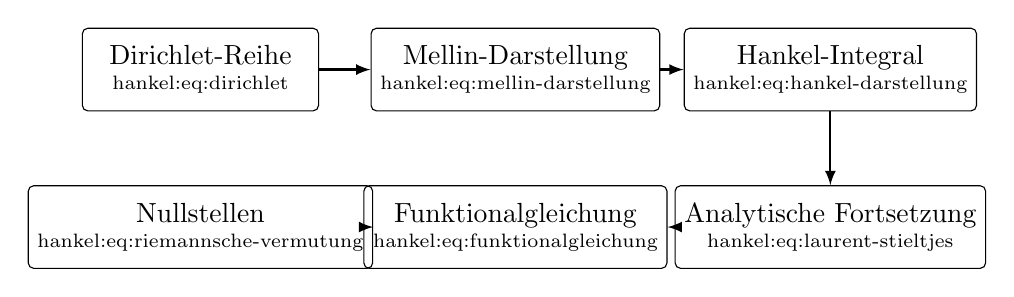
\begin{tikzpicture}[
		block/.style={
			draw,
			rounded corners=2pt,
			minimum width=3.0cm,
			minimum height=1.05cm,
			align=center
		},
		arrow/.style={->,thick,>=latex}
		]
		\node[block] (d) at (0,0)
		{Dirichlet-Reihe\\[-1mm]
			{\scriptsize\eqref{hankel:eq:dirichlet}}};
		
		\node[block] (m) at (4,0)
		{Mellin-Darstellung\\[-1mm]
			{\scriptsize\eqref{hankel:eq:mellin-darstellung}}};
		
		\node[block] (h) at (8,0)
		{Hankel-Integral\\[-1mm]
			{\scriptsize\eqref{hankel:eq:hankel-darstellung}}};
		
		\node[block] (a) at (8,-2)
		{Analytische Fortsetzung\\[-1mm]
			{\scriptsize\eqref{hankel:eq:laurent-stieltjes}}};
		
		\node[block] (f) at (4,-2)
		{Funktionalgleichung\\[-1mm]
			{\scriptsize\eqref{hankel:eq:funktionalgleichung}}};
		
		\node[block] (n) at (0,-2)
		{Nullstellen\\[-1mm]
			{\scriptsize\eqref{hankel:eq:riemannsche-vermutung}}};
		
		\draw[arrow] (d) -- (m);
		\draw[arrow] (m) -- (h);
		\draw[arrow] (h) -- (a);
		\draw[arrow] (a) -- (f);
		\draw[arrow] (f) -- (n);
	\end{tikzpicture}
	
	\caption{Der rote Faden des Kapitels.}
	\label{hankel:fig:uebersicht}
\end{figure}

%\begin{figure}
%	\centering
%	\begin{tikzpicture}[
%		block/.style={
%			draw,
%			rounded corners=2pt,
%			minimum width=3.0cm,
%			minimum height=1.05cm,
%			align=center
%		},
%		arrow/.style={->,thick,>=latex}
%		]
%		\node[block] (d) at (0,0)
%		{Dirichlet-Reihe\\[-1mm]
%			{\scriptsize\eqref{hankel:eq:dirichlet}}};
%		
%		\node[block] (m) at (4,0)
%		{Mellin-Darstellung\\[-1mm]
%			{\scriptsize\eqref{hankel:eq:mellin-darstellung}}};
%		
%		\node[block] (h) at (8,0)
%		{Hankel-Integral\\[-1mm]
%			{\scriptsize\eqref{hankel:eq:hankel-darstellung}}};
%		
%		\node[block] (a) at (8,-2)
%		{Analytische Fortsetzung\\[-1mm]
%			{\scriptsize\eqref{hankel:eq:laurent-stieltjes}}};
%		
%		\node[block] (f) at (4,-2)
%		{Funktionalgleichung\\[-1mm]
%			{\scriptsize\eqref{hankel:eq:funktionalgleichung}}};
%		
%		\node[block] (n) at (0,-2)
%		{Nullstellen\\[-1mm]
%			{\scriptsize\eqref{hankel:eq:riemannsche-vermutung}}};
%		
%		\draw[arrow] (d) -- (m);
%		\draw[arrow] (m) -- (h);
%		\draw[arrow] (h) -- (a);
%		\draw[arrow] (a) -- (f);
%		\draw[arrow] (f) -- (n);
%	\end{tikzpicture}
%	
%	\caption{Der rote Faden des Kapitels.}
%	\label{hankel:fig:uebersicht}
%\end{figure}


\section{Die Dirichlet-Reihe
\label{hankel:section:dirichlet}}
\kopfrechts{Die Dirichlet-Reihe}

Für eine komplexe Zahl $s$ mit $\operatorname{Re}(s)>1$ wird die Zetafunktion zunächst durch
\begin{equation}
\zeta(s)
=
\sum_{n=1}^{\infty}
\frac{1}{n^s}
\label{hankel:eq:dirichlet}
\end{equation}
definiert~\cite{hankel:apostol}. 
Um das Konvergenzverhalten dieser Reihe zu verstehen, muss zuerst die komplexe Potenz $n^{-s}$ genauer betrachtet werden. Da $n>0$ ist, kann hier der reelle Logarithmus ohne Mehrdeutigkeit verwendet werden:
\begin{equation}
n^{-s}
=
\exp(-s\log n).
\label{hankel:eq:komplexe-potenz}
\end{equation}
Schreibt man
\begin{equation}
s=\sigma+it,
\qquad
\sigma,t\in\mathbb{R},
\label{hankel:eq:sigma-it}
\end{equation}
so zerfällt jeder Summand in einen Betrags- und einen Phasenanteil,
\begin{equation}
\begin{aligned}
n^{-s}
&=
\exp(- (\sigma+it)\log n)
\\
&=
\exp(-\sigma\log n)\,
\exp(-it\log n)
\\
&=
n^{-\sigma}\exp(-it\log n).
\end{aligned}
\label{hankel:eq:potenz-zerlegung}
\end{equation}
Der zweite Faktor liegt auf dem Einheitskreis. 
Er verändert also nur die Phase, nicht aber den Betrag. 
Daher gilt
\begin{equation}
|n^{-s}|
=
n^{-\sigma}
=
n^{-\operatorname{Re}(s)}.
\label{hankel:eq:betrag-potenz}
\end{equation}
Abbildung~\ref{hankel:fig:komplexer-summand} zeigt diese Zerlegung schematisch. 
Für festes $n$ und $\sigma$ ist die Länge des Vektors
$n^{-\sigma}$, während der Imaginärteil von $s$ nur den Winkel
$-t\log n$ bestimmt.

%
% fig-komplexer-summand.tex
%
% (c) 2026 Prof Dr Andreas Müller
%
\begin{figure}
\centering
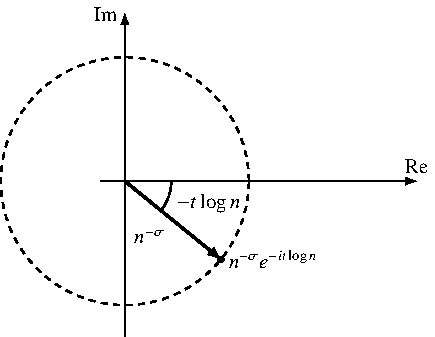
\includegraphics{papers/hankel/images/komplexer-summand.pdf}
%\begin{tikzpicture}[scale=1.05,>=latex]
%	\draw[->] (-0.4,0) -- (4.7,0) node[right] {$\operatorname{Re}$};
%	\draw[->] (0,-2.5) -- (0,2.7) node[above] {$\operatorname{Im}$};
%	\draw[dashed] (0,0) circle[radius=2.0];
%	\draw[->,very thick] (0,0) -- (1.55,-1.26)
%		node[midway,below left] {$n^{-\sigma}$};
%	\draw (0.75,0) arc[start angle=0,end angle=-39,radius=0.75];
%	\node at (1.35,-0.36) {$-t\log n$};
%	\fill (1.55,-1.26) circle[radius=1.5pt];
%	\node[right] at (1.55,-1.26)
%		{$n^{-\sigma}e^{-it\log n}$};
%\end{tikzpicture}
\caption{Betrag und Phase eines Summanden $n^{-s}$ mit $s=\sigma + it$. 
Die Darstellung ist schematisch; der Kreis hat den Radius $n^{-\sigma}$.}
\label{hankel:fig:komplexer-summand}
\end{figure}

%\begin{figure}
%\centering
%\begin{tikzpicture}[scale=1.05,>=latex]
%	\draw[->] (-0.4,0) -- (4.7,0) node[right] {$\operatorname{Re}$};
%	\draw[->] (0,-2.5) -- (0,2.7) node[above] {$\operatorname{Im}$};
%	\draw[dashed] (0,0) circle[radius=2.0];
%	\draw[->,very thick] (0,0) -- (1.55,-1.26)
%		node[midway,below left] {$n^{-\sigma}$};
%	\draw (0.75,0) arc[start angle=0,end angle=-39,radius=0.75];
%	\node at (1.35,-0.36) {$-t\log n$};
%	\fill (1.55,-1.26) circle[radius=1.5pt];
%	\node[right] at (1.55,-1.26)
%		{$n^{-\sigma}e^{-it\log n}$};
%\end{tikzpicture}
%
%\caption{Betrag und Phase eines Summanden $n^{-s}$ mit $s=\sigma + it$. 
%Die Darstellung ist schematisch; der Kreis hat den Radius $n^{-\sigma}$.}
%\label{hankel:fig:komplexer-summand}
%\end{figure}

\subsection{Absolute und lokale gleichmässige Konvergenz}

Aus \eqref{hankel:eq:betrag-potenz} folgt unmittelbar
\begin{equation}
\sum_{n=1}^{\infty}
\biggl|\frac{1}{n^s}\biggr|
=
\sum_{n=1}^{\infty}
\frac{1}{n^{\sigma}}.
\label{hankel:eq:betrag-reihe}
\end{equation}
Die rechte Seite ist dieselbe reelle Reihe wie in
\eqref{hankel:eq:dirichlet}, nun mit dem reellen Exponenten $\sigma$.
Sie konvergiert für $\sigma>1$ 
Damit ist die Dirichlet-Reihe in der Halbebene
$\operatorname{Re}(s)>1$ absolut konvergent. 
Für $\operatorname{Re}(s)\leq1$ ist sie dagegen nicht absolut konvergent; am
Punkt $s=1$ erhält man die harmonische Reihe.

Für die komplexe Analysis ist zusätzlich wichtig, dass die Konvergenz nicht nur punktweise, sondern auf kompakten Teilmengen gleichmässig ist. 
Sei dazu $K\subset\{s\in\mathbb C:\operatorname{Re}(s)>1\}$ kompakt. 
Dann besitzt $K$ einen positiven Abstand von der Geraden $\operatorname{Re}(s)=1$. 
Es gibt also ein $\delta>0$ mit
\begin{equation}
\operatorname{Re}(s)
\geq
1+\delta
\qquad
\text{für alle }s\in K.
\label{hankel:eq:kompakt-delta}
\end{equation}
Damit gilt für alle $s\in K$
\begin{equation}
|n^{-s}|
\leq
\frac{1}{n^{1+\delta}}.
\label{hankel:eq:weierstrass-majorante}
\end{equation}
Die Majorantenreihe konvergiert. 
Das weierstrasssche Majorantenkriterium liefert deshalb die gleichmässige Konvergenz auf $K$. 
Da jeder Summand $n^{-s}=\exp(-s\log n)$ als Funktion von $s$ ganz ist, ist auch die Summe holomorph. 
Die Dirichlet-Reihe definiert somit in $\operatorname{Re}(s)>1$ eine wohldefinierte holomorphe Funktion.

\subsection{Euler-Produkt und Grenze des Definitionsgebietes}

Wie in Kapitel~\ref{chapter:zeta} und in~\cite{hankel:apostol} erläutert wird, besitzt die Zetafunktion in derselben Halbebene das Euler-Produkt
\index{Euler-Produkt}%
\begin{equation}
\zeta(s)
=
\prod_{p\ \mathrm{prim}}
\frac{1}{1-p^{-s}}.
\label{hankel:eq:eulerprodukt}
\end{equation}
Die eindeutige Primfaktorzerlegung wird damit in eine analytische Identität gebracht. 
\index{Primfaktorzerlegung}%
Die Verbindung zwischen der Summe über alle natürlichen Zahlen und einem Produkt über alle Primzahlen ist ein wesentlicher Grund für die Bedeutung der Zetafunktion. 
Aus der absoluten Konvergenz des Produkts folgt insbesondere
\begin{equation}
\zeta(s)\neq0
\qquad
\text{für}
\qquad
\operatorname{Re}(s)>1.
\label{hankel:eq:nullstellenfrei}
\end{equation}
Für die weitere Untersuchung ist dieses Gebiet jedoch zu klein. 
Die Funktionalgleichung verbindet später den Punkt $s$ mit $1-s$, und die nichttrivialen Nullstellen liegen im kritischen Streifen
\begin{equation}
0<\operatorname{Re}(s)<1.
\label{hankel:eq:kritischer-streifen-einleitung}
\end{equation}
Die Dirichlet-Reihe selbst kann dort nicht einfach weiterverwendet werden.
Gesucht ist daher eine andere Darstellung, die zunächst für
$\operatorname{Re}(s)>1$ mit \eqref{hankel:eq:dirichlet} übereinstimmt, sich danach aber unabhängig von der ursprünglichen Reihe fortsetzen lässt.
Der erste Schritt in diese Richtung besteht darin, die Potenz $n^{-s}$ durch ein Integral zu ersetzen.
